\documentclass[9pt,twocolumn,twoside]{osajnl}
%% Please use 11pt if submitting to AOP
% \documentclass[11pt,twocolumn,twoside]{osajnl}

\journal{ol} % Choose journal (ao,jocn,josaa,josab,ol,optica,pr)

%See template introduciton for guidance on setting shortarticle option
\setboolean{shortarticle}{true}
% true = letter/tutorial
% false = research/review article
% (depending on journal)


\usepackage{lineno}
\linenumbers


\title{Beam focus modification by cropping partially coherent x-ray beams}


\author[1]{Manuel Sanchez del Rio}
\author[1]{Rafael Celestre}
\author[1]{Juan Reyes-Herrera}
\author[1]{Philipp Brumund}
\author[1]{Marco Cammarata}

\affil[1]{European Synchrotron Radiation Facility, 71 Avenue des Martyrs, 38000 Grenoble}

\affil[*]{Corresponding author: email@my-email.com}

\begin{abstract}
We simulate the focusing of partial coherent beams produced by fourth-generation storage rings using wave optics and coherent mode decomposition of the undulator radiation. The focus produced by a focusing system preceded an entrance slit is changed: the position is shifted and the size is enlarged with respect to those predicted by geometrical optics. This depends on the aperture used to control the coherent fraction. The pairing of two transfocators to ensure a fixed focal position is studied. Results show that the image of a partially coherent source, like an undulator in a low-emittance storage ring, is a non-trivial function of the aperture used to control the coherence fraction.
\end{abstract}

\setboolean{displaycopyright}{true}

\begin{document}

\maketitle

\section{Introduction}
\label{sec:introduction}
Fourth-generation storage-ring-based X-ray synchrotron sources deliver photon beams with high brilliance and coherence. Although the transversal coherence of these beams is highly improved in the horizontal direction, 
the overall coherent fraction is of the order of a few per cent for hard X-rays ($>10 keV$). Beamline optical elements such as pinholes and slits are then used to improve coherent fraction, to values typically $>$ 80 \% needed for applications exploiting coherence, such as X-ray photon correlation spectroscopy, coherent diffraction imaging, propagation-based phase-contrast imaging, and ptychography \cite{paganin_book}. The coherent beam interaction with the optical elements produce diffraction, thus modifying the beam characteristics and also affecting the beam focusing, as discussed here.

% This has a beneficial impact  On the other side, preserving wavefront quality requires better quality materials and optical surfaces in the active beamline components such as mirrors, gratings, crystals and lenses \cite{Yabashi, Roth2017}. Moreover,



Let us consider the case of an ideally focusing system of focal length $f$ (made by a mirror or lens that focuses the source into the image plane). The position of the focus with respect to the focusing element $q$ can be estimated by the lens equation $f^{-1}=p^{-1}+q^{-1}$, with $p$ the source-element distance. If the numerical aperture (NA) of the beam is reduced (for example by the finite dimension of the lens, mirror or by using a slit) the position and also the dimensions of the focal point changes due to diffraction. It has been shown \cite{Tanaka:85} that the focal position in a Gaussian beam ``moves" towards the lens position when the NA decreases. This shifting of the focal position is also relevant for synchrotron beamlines, as demonstrated by Westfall {\it et al.} \cite{westfahl}. These authors noticed a shift of the horizontal focal position upstream from the position given by geometrical optics (Fig. 7 in \cite{westfahl}) when the horizontal acceptance is reduced by a slit. 
% Their numeric results from wavefront propagation using SRW \cite{codeSRW} including partial coherence agree with an analytical Gaussian Shell-model.

The diffraction effect at the slits and finite size of the optical elements not only shifts the focal point, but also changes the focal dimensions. These facts are critical when designing beamlines with several coupled focusing elements. We studied this phenomenon in the context of the project for the new ID18 beamline at the upgraded EBS-ESRF storage ring. This beamline will produce highly coherent beams of variable cross section at the sample position. Two refractive systems (transfocators) will be paired to allow a varying focal size, whereas a slit placed upstream from the transfocators is used to control the coherent fraction. The optical matching of the transfocators is strongly correlated to the slit aperture (or coherent fraction). The performances of such systems are calculated applying a new fat algorithm for coherent mode decomposition (CMD) of the undulator beams, for then propagating the coherent modes. Its high efficiency is obtained implementing a 1D model, therefore studying separately the horizontal and vertical planes. The suitability and accuracy of this method is demonstrated elsewhere \cite{delrio2021pairing}.



\section{Focal image using a single lens}
\label{sec:onelens}

Let us consider an aperture of dimension $a$ placed between the source and a lens, at a distance $p_a$ from the lens ($p_a < p$). The lens is set to focus the source into an image plane at $q$ downstream from the lens. Following the geometrical optics, the position of the focal plane is not changed if the aperture $a$ changes. The focal size is $Ms$  when the aperture size $a$ is larger than the source size $s$ ($M=q/p$ is the optical magnification). But if $a<s$ the aperture obscures part of the source like if it was an ``effective" smaller source. However, the position of the waist is not modified. When the beam has a high coherence, these results predicted by geometrical optics are insufficient. This section presents numerical simulations of the focused beam (changes in focal position and focal size) when considering the partial coherent undulator emission. 
We then compute the beam evolution using wave optics. The insertion device source is a U18 undulator (period $\lambda_u=$~\SI{18}{\milli\meter}) with $N_u$~=~138 periods. The gap is tuned to have the first harmonic at $E$~=7~keV (deflecting parameter $K$~=~1.851). 

We first suppose an ideal storage ring with zero emittance, therefore producing a fully coherent emission. A Be lens of radius $R=$~ \SI{0.2}{\milli\meter} ($f=$~\SI{14.35}{\meter} at 7 keV) is placed $p=$~\SI{65}{\meter}, and a slit of variable aperture $a$ is placed at $p_a=$~\SI{29}{\meter} upstream from the lens. The beam at the slit plane has a full-width at half-maximum (FWHM) $a_\text{FWHM}=$~\SI{565}{\micro\meter}. The aperture is open at $a=n \times a_\text{FWHM}$ with different values of $n$ covering from fully opening to a very narrow aperture. The refracted beam is analyzed at different positions from the lens by calculating the FWHM of the intensity distribution. At the focal position the FWHM presents a minimum. 

\begin{figure}[htbp]
\centering
\flushleft a) {\it zero emittance}\\ \centering
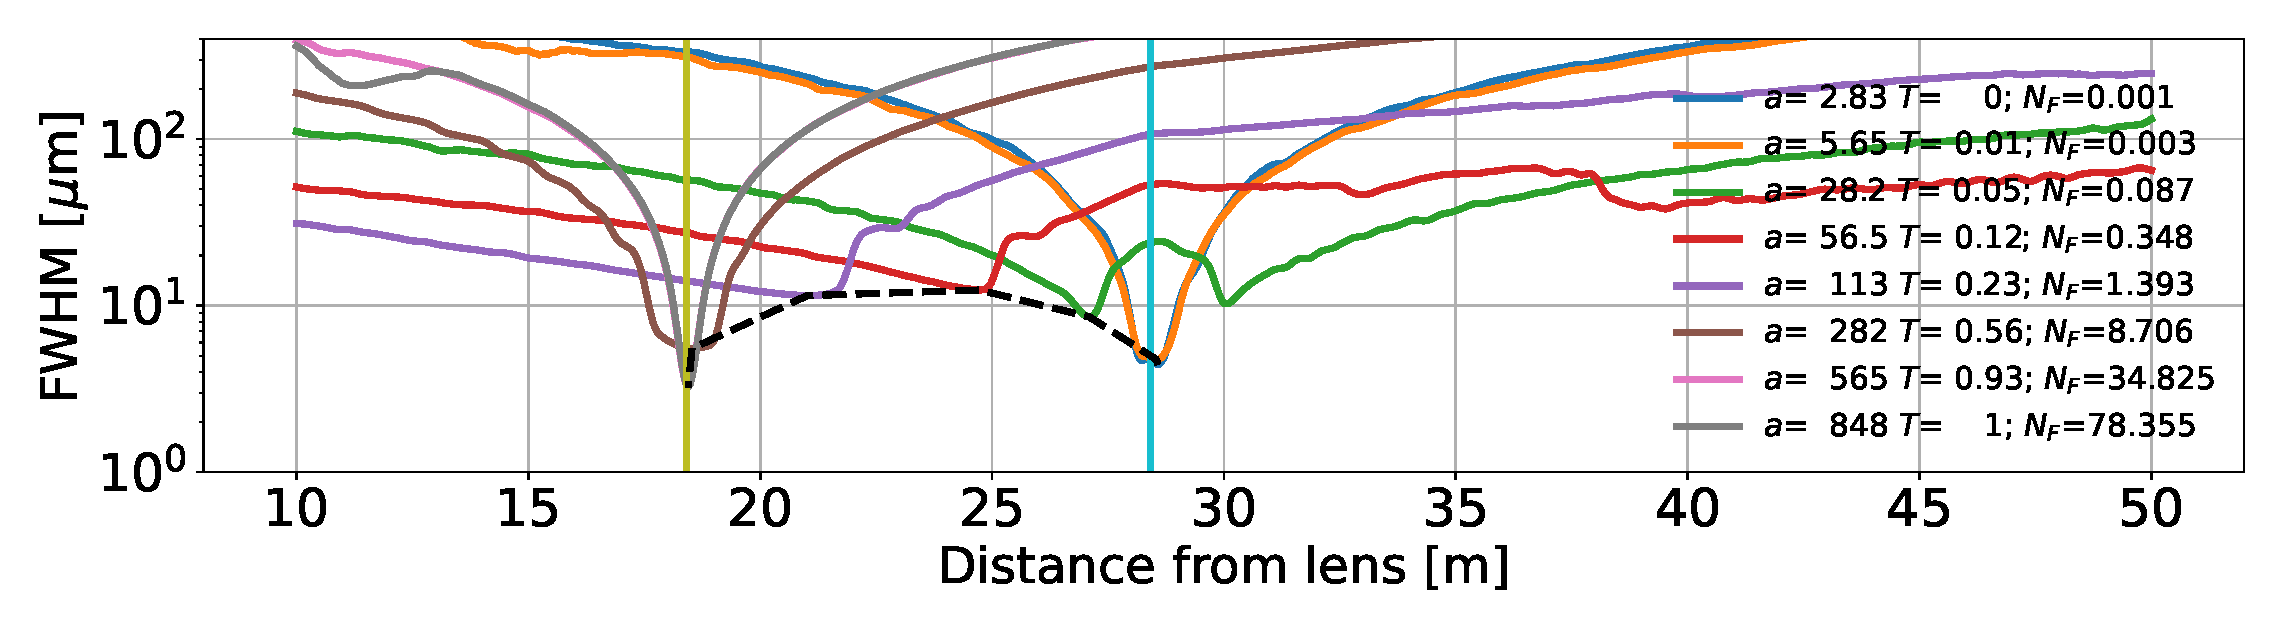
\includegraphics[width=0.45\textwidth]{figures/oneTF_UndSource_RectSlit_R200um.eps}
\flushleft b) {\it horizontal}\\ \centering
\includegraphics[width=0.45\textwidth]{figures/oneTF_UndSource_RectSlit_R200um_PartialCoherence_h.eps}
\flushleft c) {\it vertical}\\ \centering
\includegraphics[width=0.45\textwidth]{figures/oneTF_UndSource_RectSlit_R200um_PartialCoherence_v.eps}

\caption{Evolution of the size of an undulator beam cropped by a slit and focused by a lens of $R$=~\SI{0.2}{\milli\meter} 
The plot shows the FWHM of the beam  as a function of the distance from the lens. 
a) Zero emittance case (full coherence), here the aperture is open at $a = n \times a_\text{FWHM}$ for different values of $n$ (shown in the legend) and $a_\text{FWHM}$ = \SI{565}{\micro\meter} (the beam FWHM at the aperture plane). 
b) finite dimensions in horizontal (values of the ESRF-EBS emittance), and
c) finite dimensions in vertical.
Full lines in b),c) correspond to partial coherent (multimode) beam, whereas the dashed lines correspond to the full coherent beam (first mode). The coherence fraction for each slit aperture is marked in legend.
The focal positions given by geometrical optics are represented for the source placed wither at the ID position (yellow vertical line) or at the slit position (blue vertical line).
The Fresnel number $N_F$ calculated at the slit plane is also marked in the legend.
}
\label{fig:oneTFund}
\end{figure}

Fig.~\ref{fig:oneTFund}a shows the evolution of the coherent beam size after being focused by the lens. With the open slit the geometrical optics give a focal position $q=$~\SI{18.4168}{\meter} (source at the ID position, distant $p$ from the lens) and $q_a=$~\SI{28.4089}{\meter} (source at slit position, distant $p_a$ from lens). It can be noticed that for $n\ge$~1 (Fresnel number $N_F\ge$~35) the situation does not change with respect the open slit because the cropping by the slit is negligible. For $n=0.5$ ($N_F=8.7$, brown line) the FWHM of the focal size increases and the depth of focus also increases, manifested in a flat depression. For smaller values of $n$ and $N_F$ the minimum shifts to higher distances (e.g., $n=0.1$ red line) and becomes less pronounced. For $n$ = 0.05 (green line), a small beam size is found again close to the $q_a$ position, but it presents a twin minimum due to the interference fringes found in the intensity distributions. Both minima converge to a the $q_a$ position for $n\le$~0.01 (orange line). 
When the focal distance of the lens is reduced (using lenses with smaller radius, or piling several lenses), the $q$ and $q_a$ positions shift to shorter distances, and  $|q-q_a|$ also reduces. They converge to a single position: the lens focal length $q=q_a=f$. This happens when both source-lens and slit-lens distances can be considered at infinite. 

The dimension of the waist can be calculated using geometrical concepts only for the limiting cases of waist at $q$ and $q_a$. For the waist at $q$, the beam size is the source size times its magnification (ratio between lens-waist distance and lens-source distance). Similarly, for the waist at $q_a$, the beam size is the slit aperture times the magnification (now computed as the ratio between lens-waist distance and slit-lens distance). This has been verified numerically (not shown). However, for intermediate slit apertures, where the waist position is in between $q$ and $q_a$, the waist size is different to that predicted by geometric optics.
Indeed, it can be observed in Fig.~\ref{fig:oneTFund} that for these intermediate slit apertures that crop the beam, the waist size is larger than those found at limiting positions $p$ and $p_a$.
This is an important fact: A good focusing, i.e., a very small beam size is only obtained in the limiting cases of open slit and almost-closed slit. This means that for a fully coherent beam, the slit disturbs the focusing and should be avoided. The diffraction at the slit creates an an spurious divergence that affects the lens power. 

% \subsubsection{Partial coherence} The mission of the slit is to improve beam coherence (increase coherent fraction). For usual photon energies (5-25~keV)  the slit must be almost closed to gain coherence in old storage rings like ESRF-1 ($CF<10^{-3}$), thus forming a secondary source. For storage rings like EBS, with $CF > 10^{-2}$, the selection of the slit aperture $a$ is crucial: the slit must be closed until the the desired $CF$ is obtained, but not more, because it not only reduces intensity but also deteriorates the focusing. 


We used the EBS-ESRF emittance values\footnote{We used over this work the following values of electron beam sizes at the center of the straight section: $\sigma_x=~\SI{29.7}{\micro\meter}$,
$\sigma_{x'}=~\SI{4.37}{\micro\radian}$,
$\sigma_y=~\SI{5.29}{\micro\meter}$,
$\sigma_{y'}=~\SI{1.89}{\micro\radian}$, corresponding to beam emittances:  $\epsilon_x=~\SI{130}{\pico\meter \radian}$,
$\epsilon_y=~\SI{10}{\pico\meter \radian}$, and beta functions
$\beta_x=~\SI{6.8}{\meter}$,
$\beta_y=~\SI{2.8}{\meter}$
}
to perform the coherent mode decomposition of the undulator source.
This is done for the horizontal and vertical directions, resulting coherent fractions (at 7 keV) of $CF_h=$13\% and $CF_v=$58\%, for the horizontal and vertical directions. These values are much higher than for the old ESRF-1 source, but still low to justify approximating the beam by a coherent beam. Therefore, we propagated a number of modes large enough to contain more than 99\% of the source intensity (36 modes in H and 8 in V). The illumination at the entrance slit plane is \SI{610}{\micro\meter} in H times \SI{566}{\micro\meter} in V. The slit aperture is used to tune the coherence of the beam: closing the slit increases the $CF$. In the limit (zero aperture) the beam after the slit is fully coherent ($CF=1$), but obviously with zero intensity. The choice of the right slit aperture comes from a compromise between coherence and flux. 
% Figure~\ref{fig:oneTFund} shows the $CF$ after of the H and V 1D beams after the slit for different slit apertures. From this figure we select the apertures to be used in the following simulations. We selected a photon energy of \SI{7}{keV}. A first value of $CF_h=CF_v=$ 90\% in both horizontal and vertical (thus with a combined 2D  $CF=CF_h CF_v=$ 81\%) is obtained with slit apertures of
% $a_h$ =~\SI{40.3}{\micro\meter}, and 
% $a_v$ =~\SI{227}{\micro\meter} (horizontal and vertical, respectively). A second value of  $CF_h=CF_v=$ 70\% (thus 2D $CF$ of about 50\%), corresponds to 
% $a_h$ =~\SI{85.1}{\milli\meter}, and 
% $a_v$ =~\SI{506.7}{\milli\meter}. The case of the ``open" slit that does not crop the beam is also included (this is obtained, for example, with $a_h$ =~\SI{1}{\milli\meter} and $a_v$ =~\SI{1.5}{\milli\meter}).

% \begin{figure}\label{fig:oneTFundPartialCoherence}
%     \flushleft a) {\it horizontal}\\ \centering
%     \includegraphics[width=0.45\textwidth]{figures/oneTF_UndSource_RectSlit_R200um_PartialCoherence_h.eps}
%     \flushleft b) {\it vertical}\\ \centering
%     \includegraphics[width=0.45\textwidth]{figures/oneTF_UndSource_RectSlit_R200um_PartialCoherence_v.eps}

%     \caption{Evolution of the size of a coherent undulator beam cropped by a slit and focused by a lens of $R$~=~\SI{0.2}{\milli\meter} in the a) horizontal and b) vertical directions.
%     The plot shows the FWHM of the beam  as a function of the distance from the lens.
%     Full lines correspond to the partial coherent (multimode) beam, whereas the dashed lines correspond to the full coherent beam (first mode). Different slit apertures are used for obtaining different coherent fraction after the slits (marked in legend).
%     }
% \end{figure}

Figure~\ref{fig:oneTFund}b,c shows the focal size along the optical axis for these apertures in the horizontal and vertical planes. We calculated the case of the partially coherent beam (multi-mode, solid lines) and also the case of a fully coherent beam (only the first coherent mode, dashed lines). We observe that the focal positions (the minima of the plot lines) do not change significantly when passing from full to partial coherence. However, the focal dimension changes significantly in the horizontal direction for cases with $CF_h\le$ 70\%. In the vertical, where the beam at the source was more coherent there is no differences in sizes when going from full (dashed lines) to partial coherence (solid lines). Looking to the focal position shift versus slit aperture we find important differences in the horizontal and vertical. The cropping of the beam by the slit is important in horizontal as we need to increase the $CF_h$ from the source (13\%) to values required by the experiments, usually larger than 50\%. This produces a gradual shift of the focal position from the position of the geometrical image of the ID source (black line in panel a)) to the geometrical image of the slit (red line in panel a)). However, in the vertical plane, the slit crops the beam only slightly, and closing the slit to go from the source $CF_v$ = 58\% to values up to 90\% does not produce any focal shift from the position of the geometrical image of the ID source. Only when the slit is very closed (e.g., $a_v$ =~\SI{25}{\micro\meter}, red curve) the focal position shifts to the geometrical image of the slit. This case is in principle not interesting experimentally as it reduces the intensity from an already quite coherent beam ($CF_v$~= 90\%). 


\section{Focal sizes for two paired lenses}

We study here an optical system composed by two lenses (lens-1 with focal length $f_1$ and lens-2 with $f_2$) separated by a distance $D$. Following \citeasnoun{Goodman85}, the relationship between object-to-lens-1 distance $p_1$ and the lens-2-to-image distance $q_2$ is
\begin{equation}
\label{eq:twolens}
    D-(f_1+f_2)=\frac{f_1^2}{p_1-f_1} + \frac{f_2^2}{q_2-f_2}.
\end{equation}

The global magnification is the product of the magnification of the individual lenses. It can be written as
\begin{equation}
\label{eq:magnification}
    M=M_1 M_2=\frac{1-q_2/f_2}{1-p_1/f_1}.
\end{equation}

The magnification is not dependent on $D$, however the length of the optical system $L=p_1+D+q_2$ will change if one changes the focal distances of the lenses. For a constant $L$ one can change magnification by changing the inter-lenses distance $D$ (zoom effect). In a synchrotron beamline using transfocators, the magnification can be changed by varying the focal lengths of the transfocators (by adding or removing individual or group of lenses in the transfocator) \cite{Vaughan:kv5084}.

We analyze the optical design of a focusing system that uses two transfocators, and how to configure it for the desired focal size or magnification. 

\begin{table}[]
    \label{table:id18parameters}
    \caption{Position of the two transfocators, slit and sample (focal point) corresponding to the ID18 beamline configuration under study. }
    \centering
    \begin{tabular}{l|c|c}
         element & position [m] & comment\\
         ID (undulator) source& 0 & U18 $N_u$~=~138 $K$~=~1.851 (7 keV)\\
         Slit & 36 &
         variable aperture $a_h\times a_v$
         \\
         Transfocator 2D & 65 & 
         %$f_H=58.7; f_V=54.3$ 
         \\
         Transfocator 2D & 170 & $D$~=~\SI{105}{\meter} \\
        %  Transfocator 2D & 170 & position 1 {\bf FO1}, $D$=~\SI{105}{\meter} \\
        %  Transfocator 2D & 192 & position 2 {\bf FO2}, $D$=~\SI{127}{\meter}  \\
         sample & 200 & focal plane
    \end{tabular}
\end{table}

\begin{figure}\label{fig:analytical}
    \centering

    \includegraphics[width=0.25\textwidth]{figures/f1f2_analytical.eps}
    \includegraphics[width=0.25\textwidth]{figures/magnification_analytical.eps}
    \includegraphics[width=0.25\textwidth]{figures/sizes_analytical.eps}

    \caption{a) Analytical trajectories $(f_1,f_2)$ for $D$~= \SI{105}{\meter} calculated numerically [equation~(\ref{eq:twolens})] for a given value of apertures.
    b) 
    Analytical magnification \todo{$|M|$!!} calculated using equation~(\ref{eq:magnification}).
    c) 
    Analytical size values (magnification times source or slit size).
    The source is placed either at $p_1$~= \SI{65}{\meter} (source at the ID position) or $p_1$~= \SI{29}{\meter} (source at slit position). Note that cases with $f_2<0$ are not plotted as defocusing (concave) lenses are not available. 
    }
\end{figure}



\begin{figure}\label{fig:f1f2map}
    \centering

    \includegraphics[width=0.25\textwidth]{figures/f1f2_h.eps}
    \includegraphics[width=0.25\textwidth]{figures/f1f2_v.eps}

    \caption{Trajectories $(f_1,f_2)$ for $D$~= \SI{105}{\meter} calculated numerically for different values of apertures. Panel a) is for the horizontal direction and panel b) for the vertical. 
    Analytical values displayed are obtained using equation~(\ref{eq:twolens}) with $p_1$~= \SI{65}{\meter} (object at source position) (solid lines) or $p_1$~= \SI{29}{\meter} (object at slit position) (dashed lines).
    }
\end{figure}

The two transfocators in use are idealized as two real beryllium lenses of variable curvature radius $R_1$ and $R_2$ that correspond to focal distances $f_1$ and $f_2$ ($f=R/(2 \delta)$, with $\delta=$~6.96 10$^{-6}$ for Be at \SI{7}{keV}). A slit of aperture $a_h$ in horizontal and $a_v$ in vertical is placed upstream the lens-1. The positions of the elements is determined by room constraints and are considered fixed (although different values could be studied). We set the distances matching the requirements of the EBS-ESRF ID18 beamline (see Table~\ref{table:id18parameters}), and we analyzed the system at a photon energy of \SI{7}{keV}. We study the variation of the spot size as a function of the focal distances. The final goal is to get the desired focal size by selecting the configuration of the transfocators (the focal length and the particular combination of lenses to approach it). 

For fixed distances $p_1$, $D$ and $q_2$, and also a given value of $f_1$, one can calculate analytically $f_2$ using  equation~(\ref{eq:twolens}) and the corresponding magnification $M$ in the framework of geometrical optics. Taking $f_1$ as variable parameter,  
Fig.~\ref{fig:analytical}a shows the trajectories of $f_2$ as a function of a variable $f_1$. In this plot we eliminated possible values of $f_2<0$ that correspond to the second divergent (defocusing) lens, an option not available in a typical transfocator.  
The choice of one pair $(f_1,f_2)$ from these curves guarantees that the focus is at the sample position ($L=p_1+D+q_2$~= \SI{200}{\meter} from source). Fig.~\ref{fig:analytical}b shows the theoretical magnification $|M|$ and the theoretical image sizes are in Fig.~\ref{fig:analytical}c. 

Figure~\ref{fig:f1f2map} shows the value of the $(f_1,f_2)$ map calculated numerically. For each $F_1$ value, we can select from the map $f_2$ value that produces the best focus (which has a minimum FWHM or a maximum peak intensity). 

The $(f_1,f_2)$ curves depend strongly on the slit aperture in the horizontal, because of the low $CF_h$ of the source (12\%) is highly increased by the slit. In the vertical the source is more coherent ($CF_v$~=~58\%) therefore the slit improves the $CF_v$  and there is not much change in the trajectories up to values of 90\%. However, in the case of a slit with $a_v$~=~\SI{25}{\micro\meter} that is acting as a pinhole the trajectories (red line) approach the results of the geometrical optics considering the source at the slit position.

Figure~\ref{fig:focalSizes} shows the calculated focal sizes. Analytical values (dashed and dotted lines), based on geometrical optics, use  equation~(\ref{eq:magnification}). They do not reproduce correctly values of beam sizes calculated numerically with wave optics. It can be concluded that the analytical values have very limited applicability, at least in the configurations studied.
In the horizontal direction, for slit apertures $a_h>$~\SI{40}{\micro\meter} the sizes change considerably for small changes in $a_h$. The focusing characteristics of the system depends highly on the diffraction effects produced at the slit. For the slit $a_h$~=~\SI{40.3}{\micro\meter} ($CF_h=$~90\%) the focal size can vary from roughly 10 to 50 microns.  In vertical the focal size can be changed from 5 to 100 \SI{}{\micro\meter} at at $CF_v=$~90\%.

\begin{figure}
    \centering

    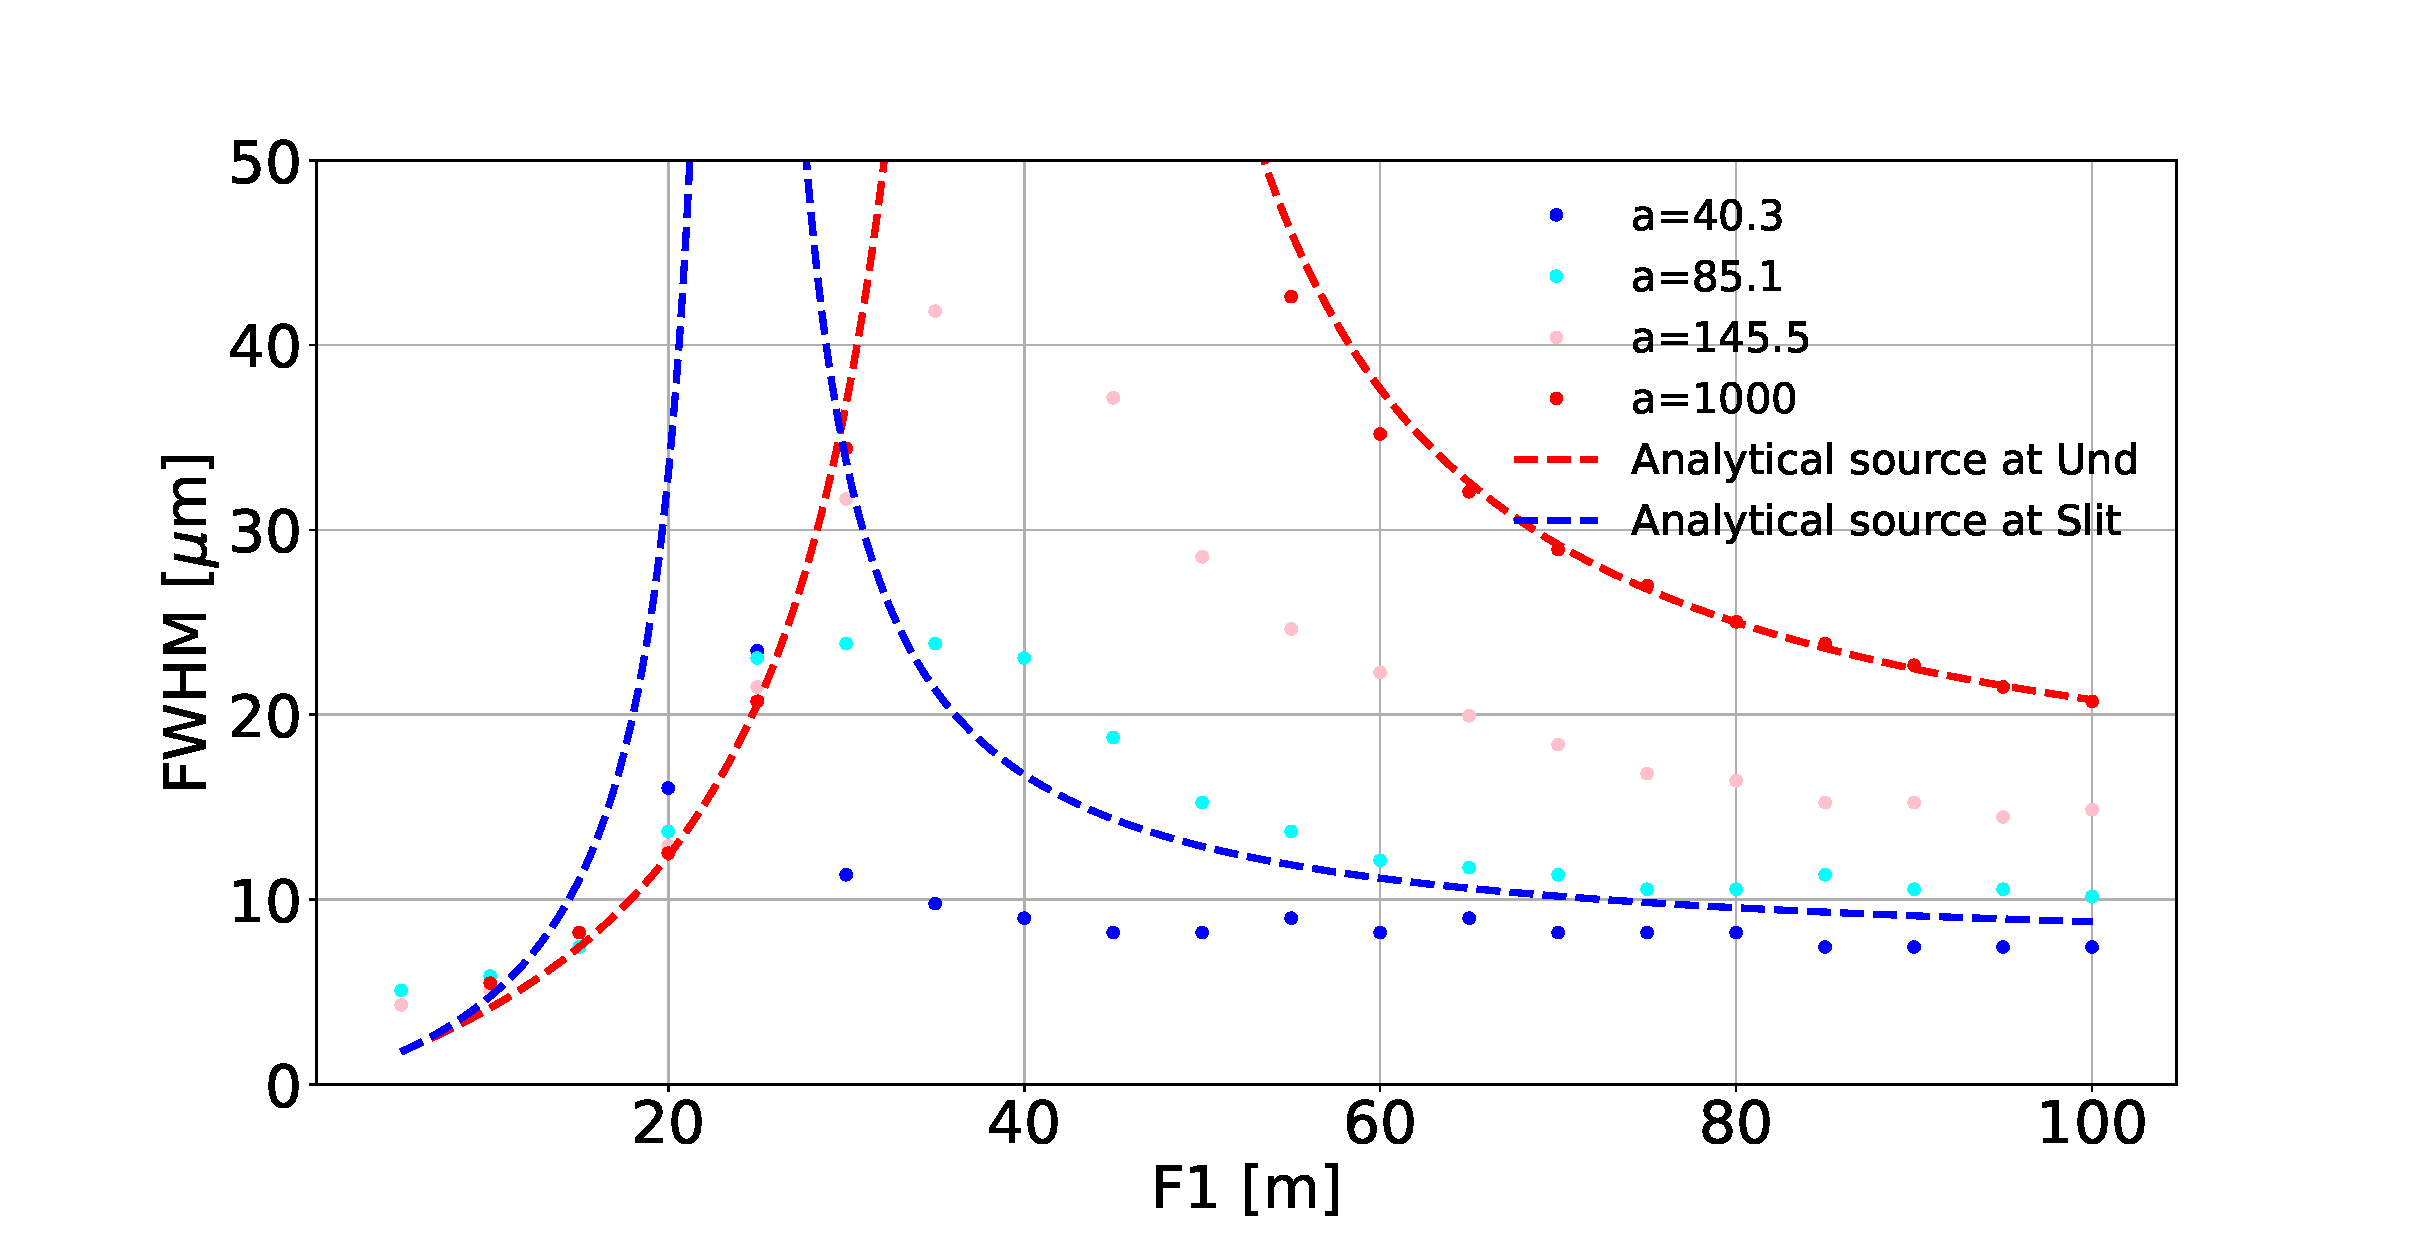
\includegraphics[width=0.25\textwidth]{figures/sizes_h.eps}
    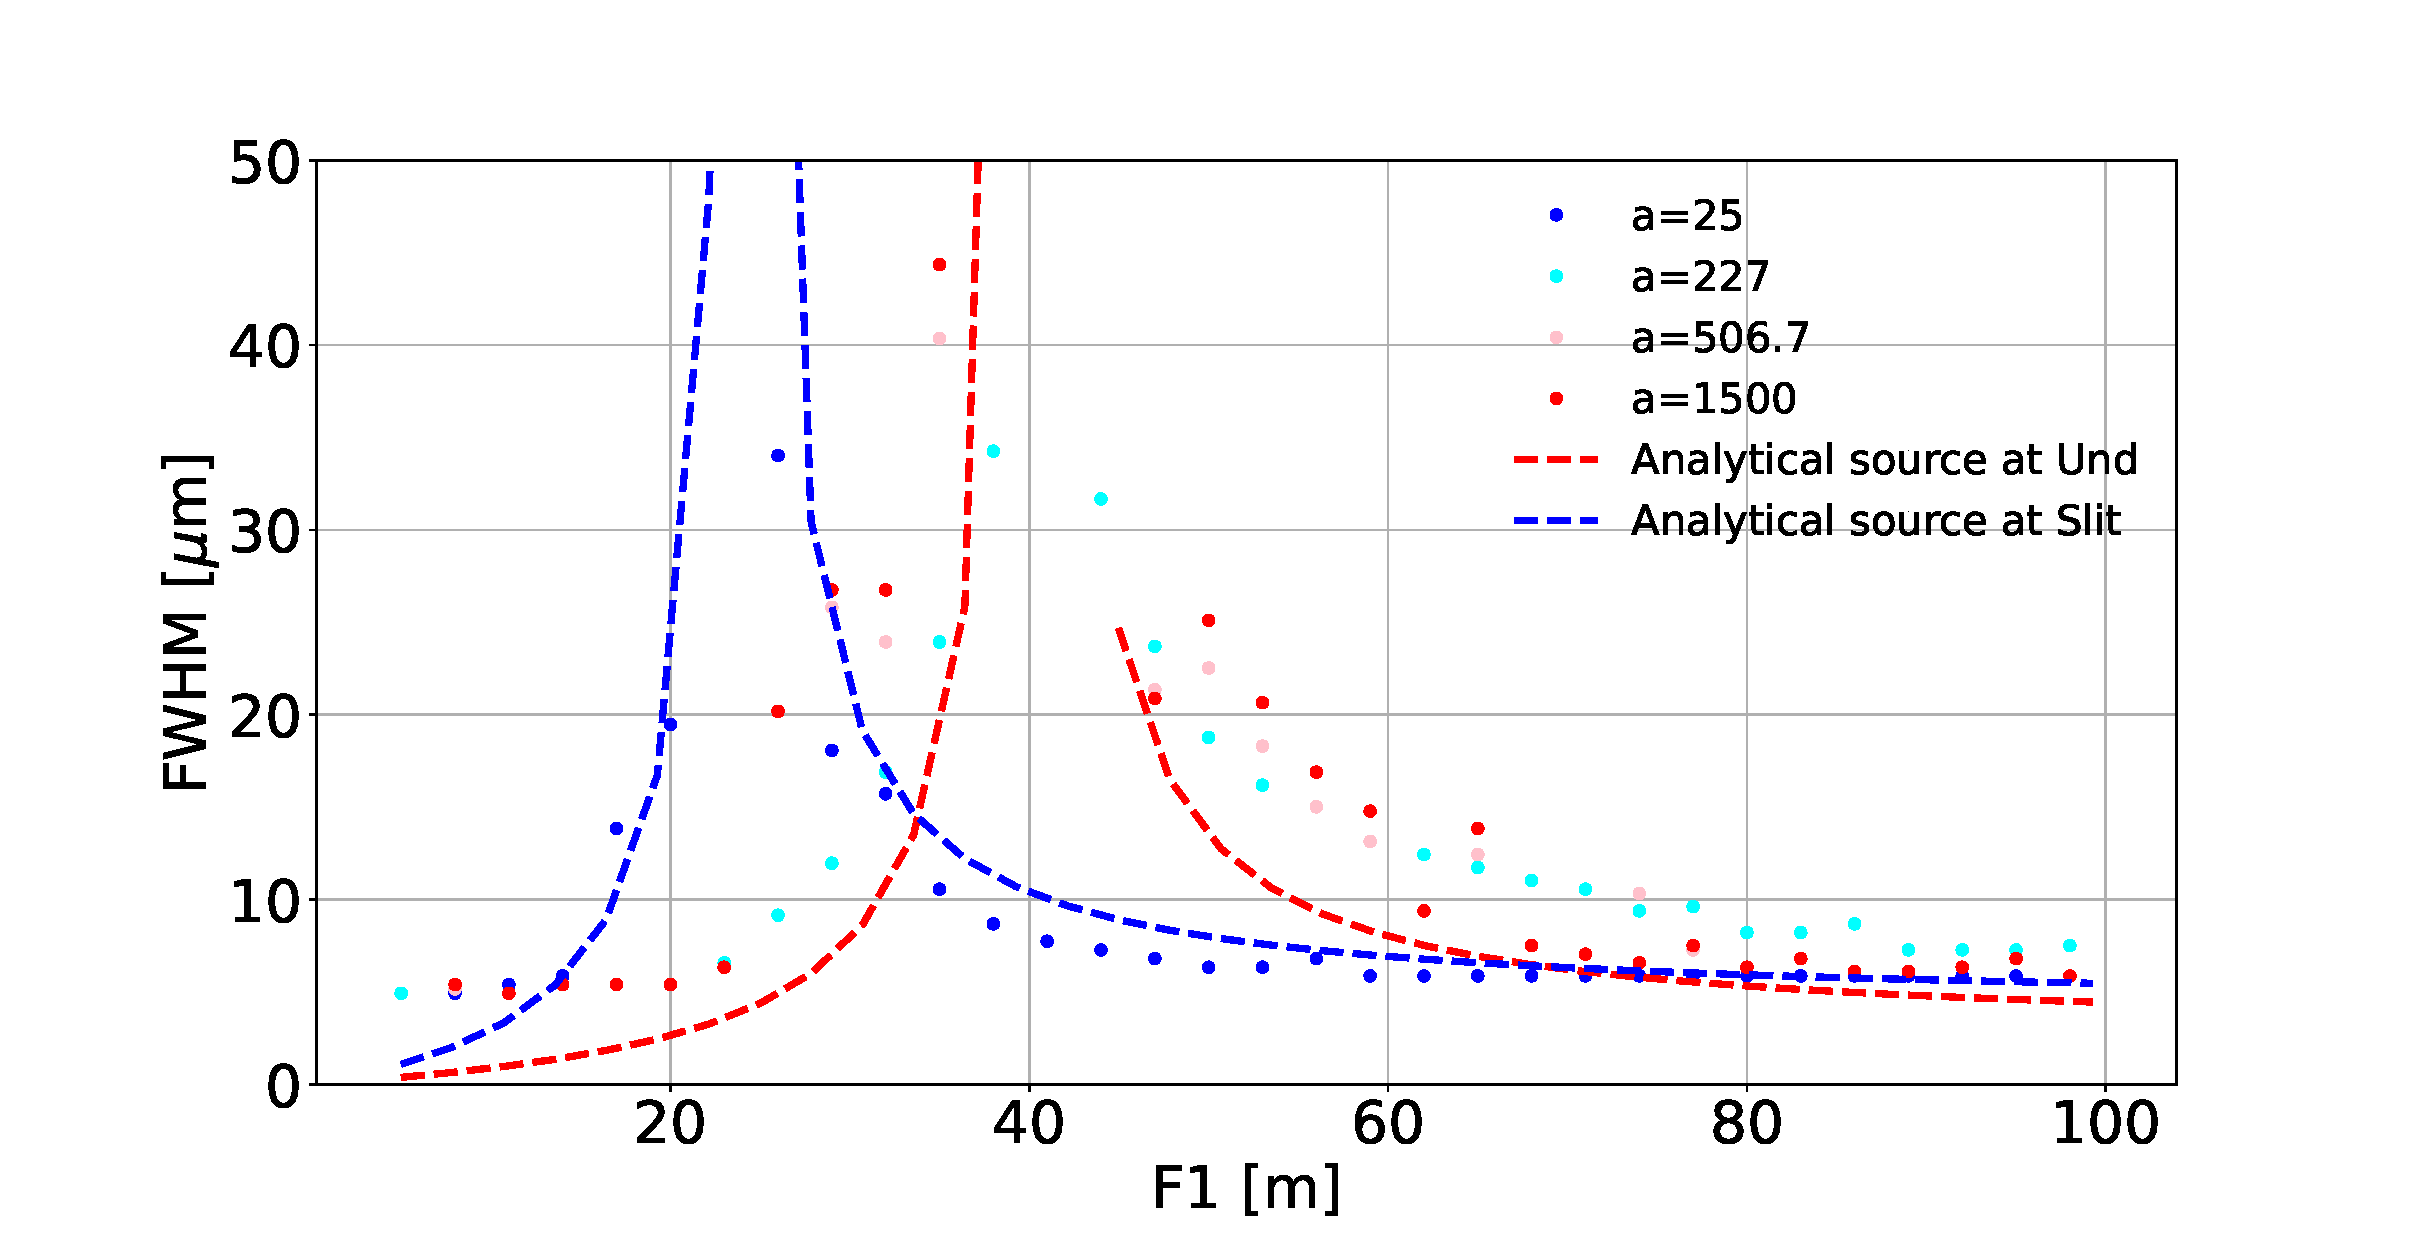
\includegraphics[width=0.25\textwidth]{figures/sizes_v.eps}
        
    \caption{Focal sizes obtained by a two transfocator system as a function of focal length of lens-1 $f_1$. The focal length $f_2$ of the second lens is obtained from the trajectories in Fig.~\ref{fig:f1f2map}. 
    Analytical values are obtained using equation~(\ref{eq:magnification}) with $p_1$~= \SI{65}{\meter} (object at source position) (solid lines) or $p_1$~= \SI{29}{\meter} (object at slit position) (dashed lines). 
    }
    \label{fig:focalSizes}
\end{figure}


% Do not place figures and tables at the back of the manuscript. Figures and tables should be placed and sized as they are likely to appear in the final article. 

% Figures and Tables should be labelled and referenced in the standard way using the \verb|\label{}| and \verb|\ref{}| commands.

% \subsection{Sample Figure}

% Figure \ref{fig:false-color} shows an example figure.

% \begin{figure}[htbp]
% \centering
% \fbox{\includegraphics[width=\linewidth]{osafig1}}
% \caption{Dark-field image of a point absorber.}
% \label{fig:false-color}
% \end{figure}

% \subsection{Sample Table}

% Table \ref{tab:shape-functions} shows an example table.

% \begin{table}[htbp]
% \centering
% \caption{\bf Shape Functions for Quadratic Line Elements}
% \begin{tabular}{ccc}
% \hline
% local node & $\{N\}_m$ & $\{\Phi_i\}_m$ $(i=x,y,z)$ \\
% \hline
% $m = 1$ & $L_1(2L_1-1)$ & $\Phi_{i1}$ \\
% $m = 2$ & $L_2(2L_2-1)$ & $\Phi_{i2}$ \\
% $m = 3$ & $L_3=4L_1L_2$ & $\Phi_{i3}$ \\
% \hline
% \end{tabular}
%   \label{tab:shape-functions}
% \end{table}

% \section{Sample Equation}

% Let $X_1, X_2, \ldots, X_n$ be a sequence of independent and identically distributed random variables with $\text{E}[X_i] = \mu$ and $\text{Var}[X_i] = \sigma^2 < \infty$, and let
% \begin{equation}
% S_n = \frac{X_1 + X_2 + \cdots + X_n}{n}
%       = \frac{1}{n}\sum_{i}^{n} X_i
% \label{eq:refname1}
% \end{equation}
% denote their mean. Then as $n$ approaches infinity, the random variables $\sqrt{n}(S_n - \mu)$ converge in distribution to a normal $\mathcal{N}(0, \sigma^2)$.

% \section{Sample Algorithm}

% Algorithms can be included using the commands as shown in algorithm \ref{alg:euclid}.

% \begin{algorithm}
% \caption{Euclid’s algorithm}\label{alg:euclid}
% \begin{algorithmic}[1]
% \Procedure{Euclid}{$a,b$}\Comment{The g.c.d. of a and b}
% \State $r\gets a\bmod b$
% \While{$r\not=0$}\Comment{We have the answer if r is 0}
% \State $a\gets b$
% \State $b\gets r$
% \State $r\gets a\bmod b$
% \EndWhile\label{euclidendwhile}
% \State \textbf{return} $b$\Comment{The gcd is b}
% \EndProcedure
% \end{algorithmic}
% \end{algorithm}

% \subsection{Supplementary materials in Optica Publishing Group journals}
% Optica Publishing Group journals allow authors to include supplementary materials as integral parts of a manuscript. Such materials are subject to peer-review procedures along with the rest of the paper and should be uploaded and described using the Prism manuscript system. Please refer to the \href{https://www.osapublishing.org/submit/style/supplementary_materials.cfm}{Author Guidelines for Supplementary Materials in Optica Publishing Group Journals} for more detailed instructions on labeling supplementary materials and your manuscript. 

% \textbf{Authors may also include Supplemental Documents} (PDF documents with expanded descriptions or methods) with the primary manuscript. At this time, supplemental PDF files are not accepted for JOCN or PRJ. To reference the supplementary document, the statement ``See Supplement 1 for supporting content.'' should appear at the bottom of the manuscript (above the References heading). 

% \begin{figure}[ht!]
% \centering\includegraphics{osafig2}
% \caption{Terahertz focusing metalens.}
% \end{figure}


% \subsection{Sample Dataset Citation}

% 1. M. Partridge, "Spectra evolution during coating," figshare (2014), http://dx.doi.org/10.6084/m9.figshare.1004612.

% \subsection{Sample Code Citation}

% 2. C. Rivers, "Epipy: Python tools for epidemiology," Figshare (2014) [retrieved 13 May 2015], http://dx.doi.org/10.6084/m9.figshare.1005064.

% \section{Backmatter}
% Backmatter sections should be listed in the order Funding/Acknowledgment/Disclosures/Data Availability Statement/Supplemental Document section. An example of backmatter with each of these sections included is shown below.

% \begin{backmatter}
% \bmsection{Funding} Content in the funding section will be generated entirely from details submitted to Prism. Authors may add placeholder text in the manuscript to assess length, but any text added to this section in the manuscript will be replaced during production and will display official funder names along with any grant numbers provided. If additional details about a funder are required, they may be added to the Acknowledgments, even if this duplicates information in the funding section. See the example below in Acknowledgements.

% \bmsection{Acknowledgments} Acknowledgments should be included at the end of the document. The section title should not follow the numbering scheme of the body of the paper. Additional information crediting individuals who contributed to the work being reported, clarifying who received funding from a particular source, or other information that does not fit the criteria for the funding block may also be included; for example, ``K. Flockhart thanks the National Science Foundation for help identifying collaborators for this work.''

% \bmsection{Disclosures} Disclosures should be listed in a separate section at the end of the manuscript. List the Disclosures codes identified on the \href{http://www.osapublishing.org/submit/review/conflicts-interest-policy.cfm}{Conflict of Interest policy page}. If there are no disclosures, then list ``The authors declare no conflicts of interest.''

% \smallskip

% \noindent Here are examples of disclosures:


% \bmsection{Disclosures} ABC: 123 Corporation (I,E,P), DEF: 456 Corporation (R,S). GHI: 789 Corporation (C).

% \bmsection{Disclosures} The authors declare no conflicts of interest.


% \bmsection{Data Availability Statement} A Data Availability Statement (DAS) will be required for all submissions beginning 1 March 2021. The DAS should be an unnumbered separate section titled ``Data Availability'' that
% immediately follows the Disclosures section. See the \href{https://www.osapublishing.org/submit/review/data-availability-policy.cfm}{Data Availability Statement policy page} for more information.

% There are four common (sometimes overlapping) situations that authors should use as guidance. These are provided as minimal models, and authors should feel free to
% include any additional details that may be relevant.

% \begin{enumerate}
% \item When datasets are included as integral supplementary material in the paper, they must be declared (e.g., as "Dataset 1" following our current supplementary materials policy) and cited in the DAS, and should appear in the references.

% \bmsection{Data availability} Data underlying the results presented in this paper are available in Dataset 1, Ref. [3].

% \item When datasets are cited but not submitted as integral supplementary material, they must be cited in the DAS and should appear in the references.

% \bmsection{Data availability} Data underlying the results presented in this paper are available in Ref. [3].

% \item If the data generated or analyzed as part of the research are not publicly available, that should be stated. Authors are encouraged to explain why (e.g.~the data may be restricted for privacy reasons), and how the data might be obtained or accessed in the future.

% \bmsection{Data availability} Data underlying the results presented in this paper are not publicly available at this time but may be obtained from the authors upon reasonable request.

% \item If no data were generated or analyzed in the presented research, that should be stated.

% \bmsection{Data availability} No data were generated or analyzed in the presented research.
% \end{enumerate}

% \bmsection{Supplemental document}
% See Supplement 1 for supporting content. 

% \end{backmatter}

% \section{References}

% Note that \emph{Optics Letters} and \emph{Optica} short articles use an abbreviated reference style. Citations to journal articles should omit the article title and final page number; this abbreviated reference style is produced automatically when the \emph{Optics Letters} journal option is selected in the template, if you are using a .bib file for your references.

% However, full references (to aid the editor and reviewers) must be included as well on a fifth informational page that will not count against page length; again this will be produced automatically if you are using a .bib file.

% \bigskip
% \noindent Add citations manually or use BibTeX. See \cite{Zhang:14,OSA,FORSTER2007,testthesis,manga_rao_single_2007}.





% Bibliography
\bibliography{sample}

% Full bibliography added automatically for Optics Letters submissions; the following line will simply be ignored if submitting to other journals.
% Note that this extra page will not count against page length
\bibliographyfullrefs{sample}

%Manual citation list
%\begin{thebibliography}{1}
%\bibitem{Zhang:14}
%Y.~Zhang, S.~Qiao, L.~Sun, Q.~W. Shi, W.~Huang, %L.~Li, and Z.~Yang,
 % \enquote{Photoinduced active terahertz metamaterials with nanostructured
  %vanadium dioxide film deposited by sol-gel method,} Opt. Express \textbf{22},
  %11070--11078 (2014).
%\end{thebibliography}

% Please include bios and photos of all authors for aop articles
\ifthenelse{\equal{\journalref}{aop}}{%
\section*{Author Biographies}
\begingroup
\setlength\intextsep{0pt}
\begin{minipage}[t][6.3cm][t]{1.0\textwidth} % Adjust height [6.3cm] as required for separation of bio photos.
  \begin{wrapfigure}{L}{0.25\textwidth}
    \includegraphics[width=0.25\textwidth]{john_smith.eps}
  \end{wrapfigure}
  \noindent
  {\bfseries John Smith} received his BSc (Mathematics) in 2000 from The University of Maryland. His research interests include lasers and optics.
\end{minipage}
\begin{minipage}{1.0\textwidth}
  \begin{wrapfigure}{L}{0.25\textwidth}
    \includegraphics[width=0.25\textwidth]{alice_smith.eps}
  \end{wrapfigure}
  \noindent
  {\bfseries Alice Smith} also received her BSc (Mathematics) in 2000 from The University of Maryland. Her research interests also include lasers and optics.
\end{minipage}
\endgroup
}{}


\end{document}
